\documentclass[12pt]{article}
\usepackage[svgnames]{xcolor}
\usepackage{tikz} 
\usetikzlibrary{arrows} 
\usetikzlibrary{calc,positioning,fit,backgrounds} 
\usetikzlibrary{decorations.pathreplacing,calc}
\usepackage{pgfplots}
\usepackage[russian]{babel}
\parskip=6pt
\usepackage{multicol}
\usepackage{amssymb, amsmath}
\oddsidemargin=-0,5cm
\textwidth=18cm
\topmargin=-3cm
\pagestyle{plain}
\textheight=25.5cm

\newcommand{\e}{\mathbb{E}}
\newcommand{\p}{\mathbb{P}}
\newcommand{\n}{\mathbb{N}}
\newcommand{\id}{\mathbb{I}}
\newcommand{\re}{\mathbb{R}}
\DeclareMathOperator{\plim}{plim}
\DeclareMathOperator{\var}{Var}
\DeclareMathOperator{\svar}{sVar}
\renewcommand{\epsilon}{\varepsilon}
\newcommand{\msum}{\sum\limits_1^n}
\newcommand{\isum}{\sum\limits_i}
\newcommand{\jsum}{\sum\limits_j}

\begin{document}
	
\begin{center}
\textbf{Перевод статьи: Tutorial on Active Inference}\\[-10mm]
\end{center}

Active inference is the Free Energy principle of the brain applied to action. It is relatively supported by experimental neuroscience studies and is a popular model of ‘how the brain works’. In this tutorial, we will consider the latest version, which is formulated as planning in discrete state-space and time. The initial motivation of active inference is that the agent wants to remain alive, by maintaining its homeostasis. To this end, the agent must ensure that important parameters, like body temperature or blood oxygenation, don’t deviate too much from the norm, i.e. are not surprising. But since it’s only possible to infer these parameters from sensory measurements, the agent minimizes surprise of sensory observations instead. Interestingly, this is equivalent to continuously improving agent’s model of the world, as we will see shortly. So in short: remain alive -> maintain homeostasis -> avoid surprising states -> avoid surprising observations -> by minimizing approximation to surprise(free energy). While the previous post aimed to give a mere intuition on Free Energy, here we will get our hands dirty. No technical background is necessary except the probability theory and Bayes Theorem. The idea goes as follows.
The brain avoids surprise by having a good model of the environment. On the one hand, the environment has a true probabilistic hidden variable (called state) s, which generates probabilistic observations o. It’s important to emphasize that the state s is hidden, meaning that we can only observe o. For example, it rained at night (s), so the grass is wet (o). This is the generative process R(s,o).

On the other hand, the brain tries to infer the probability of different hidden states given the observation, p(s|o), from the prior belief p(s) and likelihood p(o|s). Thus, the brain constructs a generative model defined as a joint p(s,o).

Let’s see a quick example. Imagine the following generative process — there is an apple and an orange tree in the garden. The identity of a fruit (apple or orange) is the hidden variable s. Suppose the apple tree is slightly to the left from the orange one, so when the fruits fall on the ground, we observe the following:

It seems like there are about 70 \% of oranges and 30 \% of apples. This is the true distribution of the hidden state s. When the fruits fall, they don’t hit the same location but somewhat randomly disperse around. This is the probability of observations conditioned on s. Inference in the generative model lies in finding posterior p(s|o) — the probability that the fruit is an apple (or orange) if it lies at a specific location. Learning the generative model consists in estimating the distributions (like parameters mean and variance for a bell-shaped Normal) of the hidden state p(s), of the state-observation mapping p(o|s). Inferring p(s|o) via Bayes formula requires us to compute p(o), which is also interesting by itself, since the better our model, the higher will be the probability of the observed data p(o). It is also called 1) ‘model evidence’, since it quantifies how well is our model predicting the real data, 2) ‘marginal likelihood’, because we marginalize, or sum out, the hidden state s. Compare 2 models below, in which we estimated p(o,s): the one on the left is obviously much better — p(s) correctly shows that there are more oranges than apples, and p(o|s) is well centered on each cluster. We can quantify the quality of each model with model evidence p(o), marginalizing the hidden variable s:

Note: technically this is a likelihood of model parameters p(o|parameters, model) and to get the actual model evidence p(o|model) we would need to marginalize over parameters as well. We'll come back to it in the end of the post.
So ideally, we want to choose model parameters that will lead to as high model evidence p(o), as possible. How does it connect to active inference and an agent that avoids surprising observations? In fact, maximizing model evidence is equivalent to minimizing surprise, which is just a negative log of p(o). If probability is 1 — surprise is 0, probability is 0 — surprise is infinite. Here is surprise as a function of probability:

And here is surprise -log p(o), overlaid with model evidence p(o):

As we discussed above for model evidence, to evaluate surprise -log p(o), we need to sum out the hidden variable s from the joint distribution p(o,s):

While this is just a summation over all possible values of s, it can be overly hard if there are many possible values of s (you’d have to sum up gazillion values). Fortunately, there is a trick to approach this impossible summation.
Instead of computing surprise directly, we can approximate it by something that is close enough, but much easier to work with. First, we introduce a dummy distribution q over the space of s (which will turn out really useful later). We could safely bring it inside the summation by multiplying and dividing at the same time:

This gives us a weighted sum, where for each s, the ratio p(o,s)/q(s) is weighted by q(s). It is still the same surprise -log p(o), but now, we are in a good shape to replace it by an approximation.
Now let’s put surprise aside for a second, and reflect on a possible approximation. We know that the function of surprise -log looks like a valley or a bowl (i.e. it is convex). Colloquially, the definition says: the function is convex if, when you drop a stick on it, the stick gets trapped in the function like in a bowl. We express this idea formally as follows. Let’s take 2 points in the function’s domain (x and y), and pick a number between 0 and 1 (w). As pictured below, we can move between x and y by computing the weighted sum and changing w from 0 to 1. So you could consider w and (1–w) as parameters of a simple distribution. Actually, there is a short name for ‘weighted sums, in which the weights are defined by a distribution’ — expectation. Now back to the stick in a bowl: if you evaluate the function of this expectation, it will always be lower or equal to the expectation of the function evaluated at x and y.

Since we earlier expanded surprise as a function (-log) of the expectation (weighted sum of the ratio p(o,s)/q(s)), it looks suitable for our approximation, following this inequality of convexity! Formally, it’s called ‘an upper bound’, a quantity that approaches from above. Lo and behold, this upper bound is…the Free Energy:

We could go a step further and remove the minus in front of the log. This brings us to the definition used in Active Inference papers.

The cool thing about Free Energy is that weights in the summation are defined by q(s), and we have a full control over q(s). So basically we can wiggle q(s) in a way that minimizes Free Energy.
Using a couple of standard identities, Free Energy (usually appended with ‘Variational’ in the literature) can be decomposed in 2 equivalent ways.

While the right branch is usually used in practice, let’s focus on the left one, as it gives us a nice theoretical insight [note: we can remove expectation (the sum over s of q(s)) in front of -log p(o), because p(o) does not depend on s, and q(s), as a probability distribution, sums up to 1]. It says that Free Energy is equal to KL (Kullback — Leibler) divergence between q(s) and p(s|o), and surprise -log p(o).

KL divergence quantifies how different are 2 distributions. For example, if a distribution p over coin landing head or tail is [0.5, 0.5] and another distribution q is also [0.5, 0.5], KL divergence is 0.
So by minimizing Free Energy, the arbitrary distribution q(s) gets closer to the posterior p(s|o), and if they match, KL term becomes 0 and Free Energy is exactly equal to surprise. So the more we minimize Free Energy by wiggling q(s), the more it becomes closer to surprise (since it’s an upper bound), and by minimizing Free Energy by wiggling parameters of p(o,s) we can minimize surprise even further. This is illustrated in detailed in the post on predictive coding, which is a corollary of the Free Energy principle applied to perception. Here is the summary so far: minimize approximation to surprise (free energy) -> avoid surprising observations -> avoid surprising states -> maintain homeostasis -> remain alive
So far, we dealt with a static situation, with one hidden state and one set of observations, but the real world is dynamic. So we would have a hidden state at each point in time, and since things tend to depend on what has just happened before, we'll assume that s at a certain time t depends on s at the previous time point. For example, a probability of seeing a rainbow depends directly on whether it rained before.

As before, we try to model the true generative process by learning a generative model p(o,s) and obtaining an approximation to the posterior q(s) at each time step. As in a simple static situation, we can find in which direction to change the parameters of p(o,s) and q(s) to decrease the Free Energy, and then make many little steps in that direction.

This would work, but we would be just passively observing the environment. What if we also act on it? In this case, s at a certain time t would depend on the s at the previous time point and our action u. In other words, action can directly affect the state of the world, so a different action would lead to a different future (e.g. we can physically move things by our actions).

Now the inference becomes active! We just have to find a way to choose a good action at each time step. In reality, it seems that we don't consider consequences of action at only next time step, but we plan the whole policy, a series of action, oriented towards goals that are distant in time. So if there are many possible actions and many future time points -> there are many potential policies we can undertake. Active inference says: just consider all of them. So we do the inference, approximating p(s|o) with q(s), simultaneously (in parallel) for every possible policy pi.

And since our goal is still the same - to minimize surprise by minimizing the Free Energy - we can compute the Free Energy (and the direction to change q(s) that will minimize FE) under each possible policy and time step.
Policies that minimize Free Energy in the future are preferred. Let's say we plan for 10 time steps ahead. If we are at time t=1, for each policy, we sum up the Free Energies for time steps 1 to 10, and pick a policy that has a minimum cumulative Free Energy in the future. Let's see again the big picture of how Free Energy can be calculated:

The left branch shows us important theoretical properties of Free Energy minimization (e.g. that q(s) approaches p(s|o)), but it is impractical, since we use Free Energy to approximate -log p(o) in the first place. So let's look on the right branch, which is a standard way to compute Free Energy:

These 2 terms are usually called Complexity and Accuracy. Complexity indicates how much the approximation of the posterior q(s) deviates from the prior p(s), and quantifies how many extra bits of information that are not in the prior we want to encode in the approximate posterior q(s). Accuracy (expected p(o|s)) scores how likely are states s given a specific outcome o. While we can easily compute the Complexity term, there is a problem in estimating Accuracy for the future time steps — simply because we haven't observed the outcomes yet. Thus, we need another way to compute the Free Energy, so we'll go by the left branch of FE decomposition. But here is a catch: since we don't have access to future observations — we'd have to guess what they could look like, and take the weighted sum of the Free Energy over the guesses p(o|s). Note, we will condition probabilities on pi, since Free Energy is estimated separately for every policy. Only state-observation mapping p(o|s) is assumed to be the same for all policies.
\newpage
\subsection{Liza's part}

Итак, нам нужно предсказывать как будущие состояния $q(s|\pi)$, так и наблюдения. А также оценивать свободную энергию на их основе. Давайте пройдем шаг за шагом, сначала сосредоточившись на знаменателе $p(o,s|\pi)$. Рассматривая левую ветвь разложения свободной энергии, показанную выше, мы можем преобразовать ее так же, как $p(s|o) \cdot p(o)$:

%So we will have to predict both future states q(s|pi) and observations, and to estimate the Free Energy based on that. Let's go step by step, first focusing on the denominator p(o, s|pi). Following the left branch of Free Energy expansion shown above, we can split it as p(s|o) p(o):

\begin{figure}[h]
	\centering{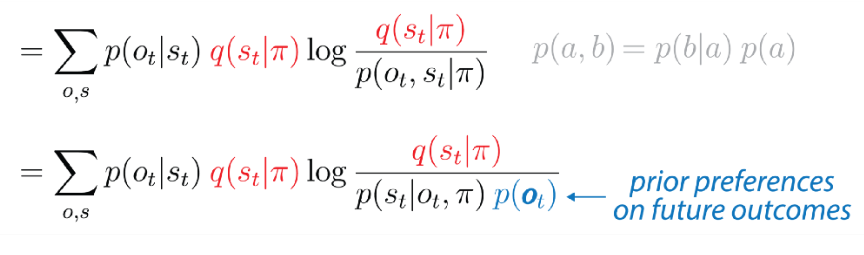
\includegraphics[width=0.8\linewidth]{1.png}}
\end{figure}

$p(o)$ - это the prior preference on the future outcomes (которое пропорционально вознаграждению в классическом обучении с подкреплением). Разделив логарифм, мы получаем следующие две величины:  отрицательное эпистемическое (т.е. знание) значение (negative epistemic value) и ожидаемое предшествующее предпочтение (expected prior preference):

%The term p(o) is the prior preference on the future outcomes (which is proportional to reward in classical reinforcement learning). We will see how it will play out later. Splitting the log, we get the following 2 terms — negative epistemic (i.e. knowledge) value and expected prior preference:

\begin{figure}[h]
	\centering{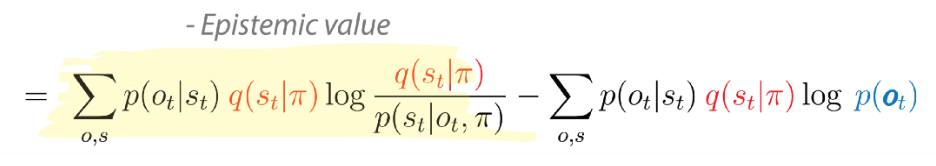
\includegraphics[width=0.8\linewidth]{2.png}}
\end{figure}

Короче говоря, эпистемическое значение (epistemic value) говорит нам, насколько будущие наблюдения могут уменьшить нашу неопределенность относительно аппроксимации апостериорного $q(s)$ (the approximate posterior q(s)). Давайте сначала закончим вывод, а затем обсудим его подробно. У нас есть истинное апостериорное $p(s|o,\pi)$ в знаменателе левого слагаемого, которое, как мы знаем, трудно вычислить, особенно в будущем (имейте в виду, что мы предсказываем будущие состояния и наблюдения). Таким образом, мы могли бы применить формулу Байеса, чтобы повторно выразить это соотношение в более вычислимых выражениях:

%In brief, epistemic value tells us how much future observations can decrease our uncertainty over the approximate posterior q(s). Let's finish the derivation first and then discuss it in detail. We have the true posterior p(s|o,pi) in the denominator of the left term, which we know is hard to compute, especially in the future (keep in mind that we are predicting future states and observations). So we could apply Bayes formula to re-express that ratio in more computable terms:


\begin{figure}[h]
	\centering{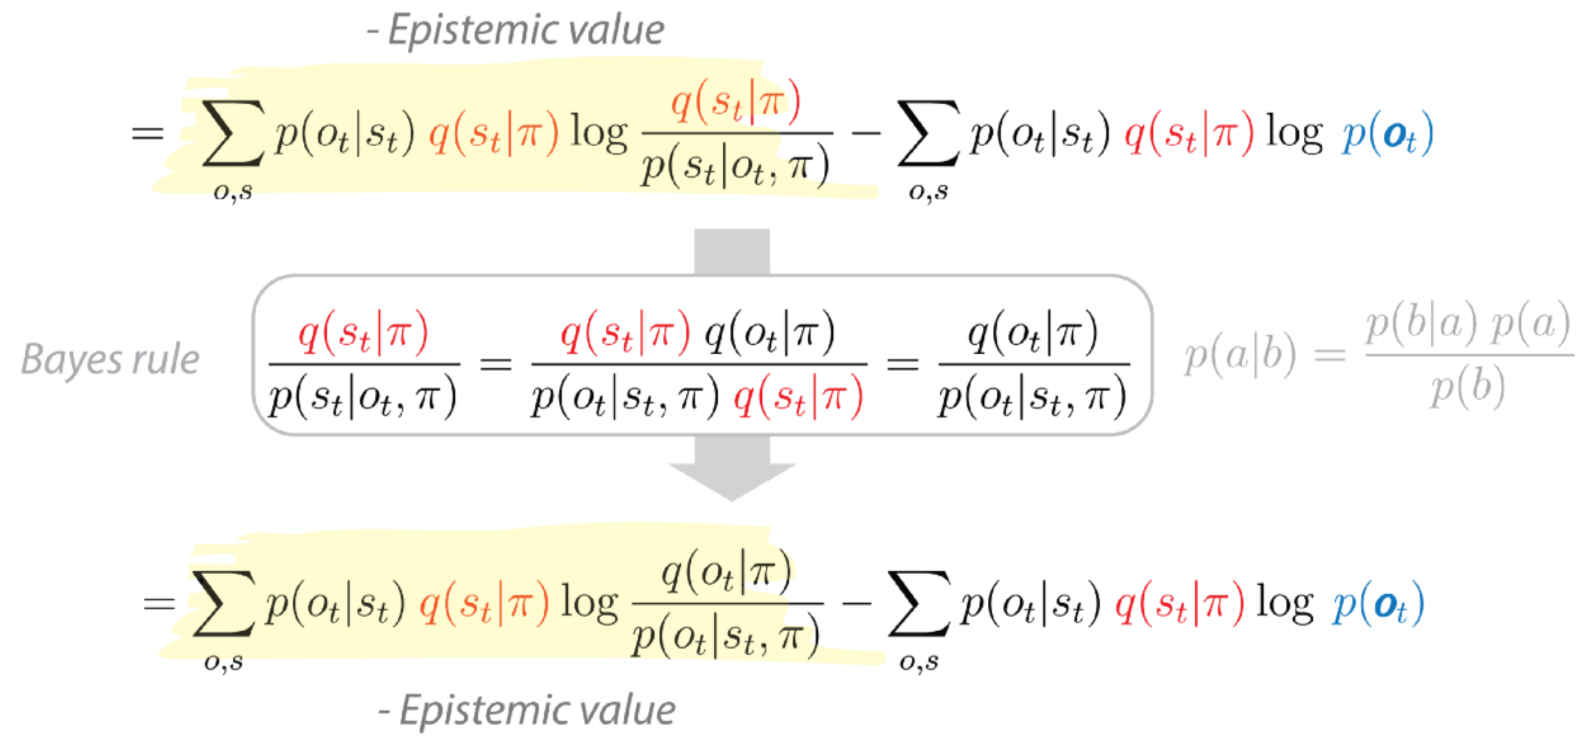
\includegraphics[width=0.8\linewidth]{3.png}}
\end{figure}

Это было бы легче сделать, если бы вы пренебрегли зависимостью от $\pi$. Тогда $q(o)$ это вроде маргинального распределения (marginal likelihood), $p(o|s)$ -- вероятность (likelihood) и $q(s_t|\pi)$ -- априорное распределение (?). Вы также можете заметить, что для некоторых распределений <<$p$>> заменяется на <<$q$>>. Это результат аппроксимации, так как, например, $p(s|o,\pi)$ является истинным апостериорным распределением, которое мы можем аппроксимировать с помощью $q(s|o,\pi)$, что при разложении приведет к тому, что все компоненты формулы Байеса будут формой $q$. Также обратите внимание, что $q(o|s,\pi)$ это то же самое, что и $p(o|s,\pi)$, поскольку это все еще относится к той же вероятности (likelihood).

%It could be easier to follow if you disregard the dependence on pi. Then, q(o) is like marginal likelihood, p(o|s) is the likelihood, and q(s_t|pi) is the prior. You may also notice that ‘p’s get interchanged with ‘q’ for some distributions. This is a result of approximations, since, for example, p(s|o,pi) is a true posterior distribution which we can approximate with q(s|o,pi), which, when expanded, would yield all components of Bayes formula to be q. Also note that q(o|s,pi) is the same as p(o|s,pi) since it’s still referring to the same likelihood.

Мы также могли бы объединить логарифмы и снова разделить их по-другому, что приводит нас к окончательной форме ожидаемой свободной энергии:

%We could also combine the logs and split again in a different way which brings us to the final form of expected Free Energy:

\begin{figure}[h]
	\centering{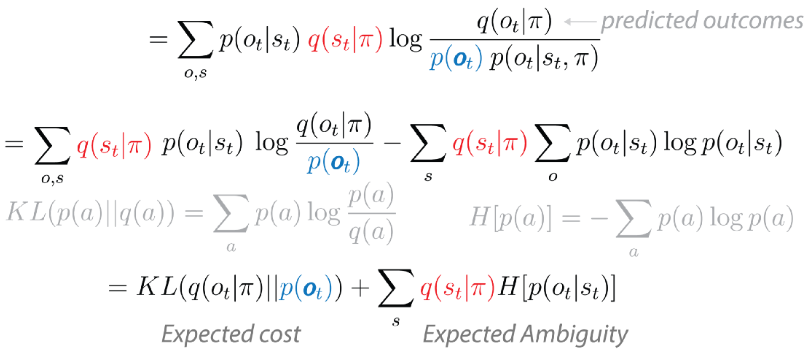
\includegraphics[width=0.8\linewidth]{4.png}}
\end{figure}

Примечание: на левой стороне мы можем повторно выразить $q(s|\pi) p(o|s)$ как совместное распределение $q(s,o)$ и просуммировать по всем $s$, чтобы получить $q(o)$. Это даст нам ожидаемую дивергенцию Кульбака-Лейблера. А на правой стороне мы можем удалить $\pi$ из $p(o|s,\pi)$, потому что вероятность (likelihood) одинакова для каждой политики.

%note: on the left side, we can re-express q(s|pi) p(o|s) as a joint q(s,o), and marginalize s to get q(o), giving us the expected KL divergence; and on the right side, we can remove pi from p(o|s,pi) because likelihood is the same for every policy

Левое слагаемое (называемое "Издержки" или "Риск") -- это дивергенция Кульбака-Лейблера между двумя распределениями: ожидаемыми в рамках политики $\pi$ наблюдениями $q(o|pi)$ и априорными предпочтениями (prior preferences). Таким образом, минимизация ожидаемой свободной энергии будет способствовать политике, которая приведет к наблюдениям, которые нам нравятся. И правое слагаемое, неоднозначность (Ambiguity), количественно определяет, насколько неопределенным является отображение между состоянием и наблюдениями $p(o|s)$. И это окончательная формула свободной энергии в будущем. Давайте теперь посмотрим на эпистемическое значение (слагаемое, которое появилось раньше, окрашено в желтый цвет).

%The left term (called 'Cost' or 'Risk') is the KL divergence between 2 distributions: expected observations under the policy pi q(o|pi) and prior preferences. So minimizing expected Free Energy would favor policies that will result in observations we like. And the right term, Ambiguity, quantifies how uncertain is the mapping between state and observations p(o|s). And this is the final formula of Free Energy in the future. Let's look on epistemic value now (the term that appeared earlier, colored in yellow).

Эпистемическое значение говорит нам, как много мы могли бы извлечь из окружающей среды, если бы следовали этой политике. Так происходит потому, что эпистемическое значение представляет собой взаимную информацию (mutual information) между скрытыми состояниями $s$ и ожидаемыми наблюдениями $o$. Взаимная информация количественно определяет, насколько неопределенность ($H$) по одной переменной уменьшается, если мы знаем другую.

%Epistemic value tells us how much we could learn from the environment if we followed this policy. This is because epistemic value is a mutual information between the hidden states s and expected observations o. And mutual information quantifies how much uncertainty (H) over one variable decreases if we know the other.

\begin{figure}[h]
	\centering{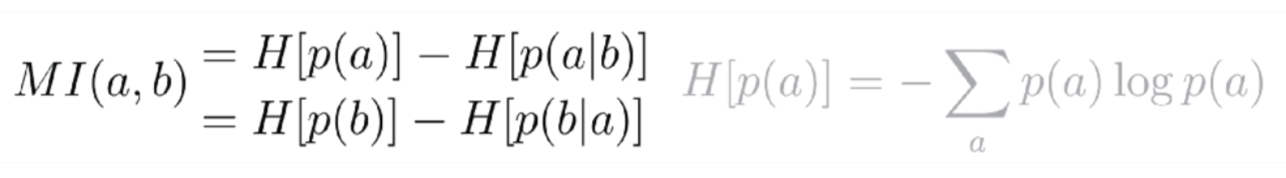
\includegraphics[width=0.8\linewidth]{5.png}}
\end{figure}

Аналогично, взаимная информация может быть повторно выражена как дивергенция Кульбака-Лейблера между совместным распределением двух переменных (если взаимная информация велика, то знание одной переменной говорит нам много о распределении другой) и произведением их маргинальных плотностей (marginals) (как если бы они были полностью независимы). Нам просто нужно перевернуть номинатор и знаменатель (потому что эпистемическое значение отрицательно в уравнениях). Обратите внимание, что мы можем удалить $\pi$ из $p(o|s, pi)$, потому что вероятность одинакова для каждой политики.

%Equivalently, mutual information can be re-expressed as the KL divergence between a joint distribution of 2 variables (if MI is high, knowing one variable tells us a lot about the distribution of the other) and product of their marginals (as if they were completely independent). We just need to flip nominator and denominator (because epistemic value is negative in the equations). Note, we can remove pi from p(o|s,pi) because likelihood is the same for every policy.

\begin{figure}[h]
	\centering{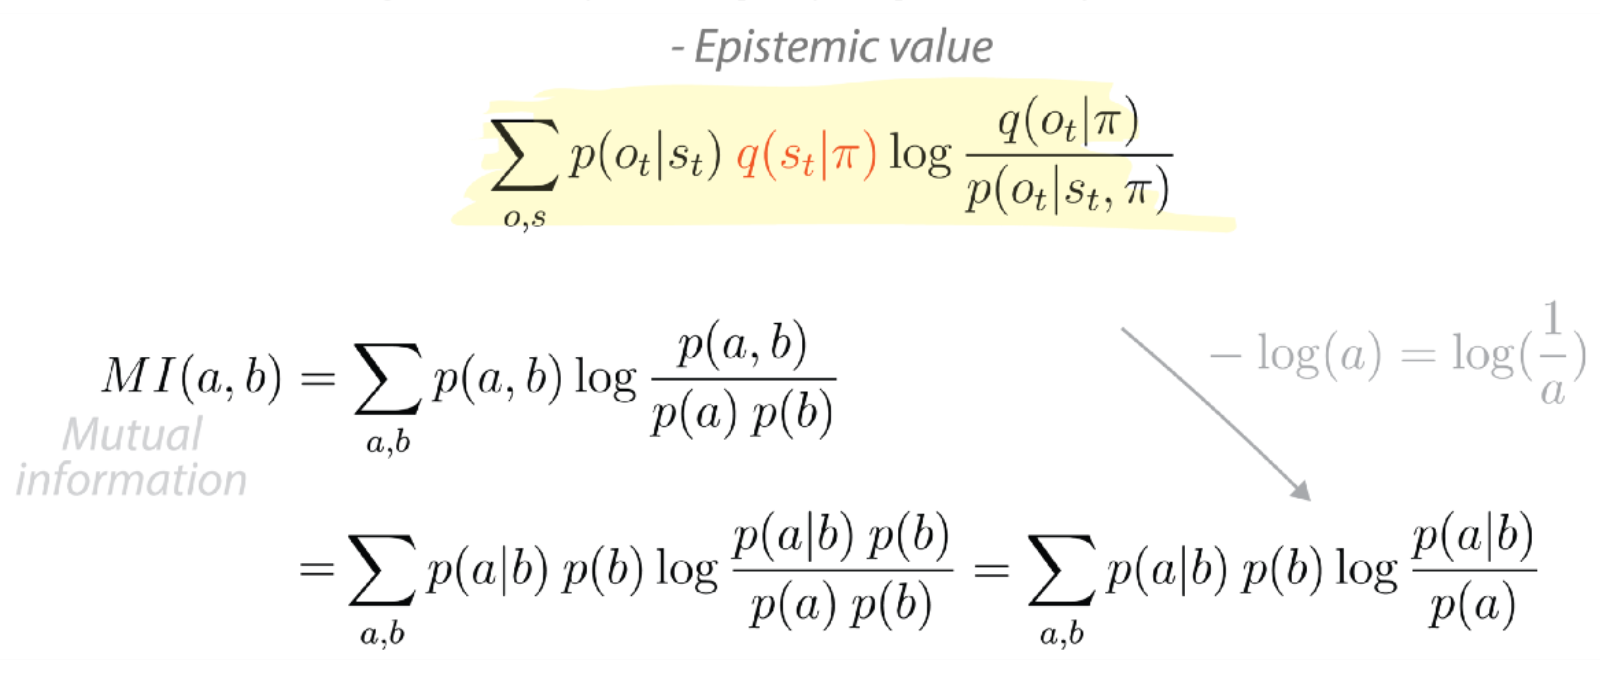
\includegraphics[width=0.8\linewidth]{6.png}}
\end{figure}

На практике эпистемическое значение зависит от неопределенности относительно будущих состояний $q(s|\pi)$. Если вы абсолютно уверены, тогда $H[q(s|\pi)]$ невелико, вам больше нечему учиться, поэтому эпистемическая ценность будет низкой. Но если вы не уверены, $H[q(s|\pi)]$ высоко, и существует сильная зависимость между состояниями и наблюдениями (поэтому $H[q(s|o)]$ низок), то взаимная информация будет высокой (см. формулы взаимной информации в терминах энтропий выше). Надеюсь, что прочитав приведенным описаниям несколько раз и пройдя их самостоятельно, оно станет простым.

%Practically, epistemic value depends on the uncertainty about future states q(s|pi). If you are very certain, H[q(s|pi)] is small, there is nothing more to learn, so epistemic value will be low. But if you are uncertain, H[q(s|pi)] is high, and there is a strong dependency between states and observations (so H[q(s|o) is low), then mutual information will be high (see MI formulas in terms of entropies above). Hopefully, going through the passages a few times and deriving them yourself, will make it straightforward. Regarding the interpretations of various Free Energy terms, they are discussed at lengths in the papers.

Here is a minimalistic example of what would actually happen inside agent's brain, if it were to use active inference. For simplicity, suppose the environment has only two states s : "1" and "2", for example, there is food in your stomach (1) or not (2). Similarly, there are only two possible observations o: "1" and "2", you feeling fed (1) or hungry(2). Suppose we already know the parameters of the generative model p(o,s). The likelihood (called "A" matrix) p(o|s) maps states to observations — if you have food — you are fed and vice versa. The transition probability p(s\_t|s\_t-1,u) maps the previous state to the next one. But since the transition also depends on action u, we can express it as a separate transition matrix ("B") for each action. Suppose we can either go get food (u1) or do nothing (u2). So if we pick u1 — we will have food in the next state, regardless of whether we have it now, and vice versa. Finally, we also have prior preferences p(o) — we like to be fed and not hungry, so we assign a higher probability to observation "1" — fed. In other words, we express preferences over observations as probability p(o).

Now imagine we observe that we are hungry and have to plan our actions for the next 2 time steps.

Since there are only 2 possible actions and 2 time steps, we can evaluate all possible policies: 11 (go for food in both time steps), 12, 21, 22. In fact we will estimate the posterior distribution on the future states (whether the food will be in our stomach), under each of these policies:

Since we know how the states are related to observations (p(o|s), 'A' matrix), we can estimate the predicted observation for each policy q(o|pi), and compute the KL term (shaded in blue below) of the expected Free Energy. Similarly, we can also evaluate the Ambiguity term (shaded in orange below), which depends on p(o|s):

Then, we'd sum the expected Free Energy over future time steps and transform it into a probability distribution over policy q(pi). So the smaller the Free Energy — the higher the probability of the policy. Interestingly, during the transformation, Free energy is weighted (i.e. multiplied) by precision, that determines how much we are confident about the beliefs over policies (i.e. by changing precision to its extrmes, our beliefs can collapse on a single policy or spread uniformly). This is imporant to determine exploration/exploitation, as the more confident you are that you have a good policy (i.e. high precision), the less you explore and vice versa.

Now you could just pick the policy that minimizes Free Energy the most, but, there is a neater way: instead of selecting 1 policy, we would do averaging over them. Think of it as if at a certain time point, there was one policy that would yield the lowest Free Energy, and other policies would be just slightly worse. As you receive new observations over time, it may turn out that the globally best policy was among those that were 'slightly worse' before. But what if you already selected an action that precludes you to follow this newly discovered policy? Thus, we let every policy vote during action selection, with the policies that minimize Free Energy the most, having the biggest weight. We take the expectation of q(s|pi) under q(pi) — a weighted sum, where the weights are defined by the probability of each policy. This results in a marginal distribution q(s), which incorporates the policy (and hence expected FE) implicitly.

And now, we are ready to act! We pick the action that minimizes the difference (KL divergence) of what we expect to see in the next time step, and what we were to see if we picked a specific action. First, to get the (probability of) expected observations, we multiply our belief on the hidden state at the next time step q(s\_t+1) by the state-observation mapping p(o|s) ('A' matrix):

And to get the expected observations if we were to take a certain action, we take our belief on the hidden state at the current time step q(s\_t), multiply it by the action-specific state-transition matrix B (to get the hypothetical next state), and then by state-observation matrix A (to get the hypothetical observation). The action that minimizes the KL divergence is executed, generative process returns us the next observation at time t+1, and the process starts again. And that is it.

So to sum up, we never actually model the action directly, but instead: estimate the hidden states under each policy -> evaluate expected free energy for each policy -> transform it to probability of policies -> average states over policies, and finally, -> act such as we observe what we expect.
Formally, associating probability of each policy with expected FE "G" is done as follows. First, the model p(o, s) actually also includes the policy, looking more like p(o, s, pi). Similarly, the approximate posterior q also includes the policy and looks like q(s, pi). Then, the solution to the optimal policy is shown analytically, and in addition to expected FE G, include the prior preferences on the policy p(pi) and the Free Energy of the past time steps (where we actually can evaluate the Accuracy term since the observations are already known). However, if we assume that all policies in the past are the same — composed of actions already performed — approximate posterior on policies q(pi) indeed depends only on expected FE G in the future. Minimizing free energy in the future is a ‘hard-coded’ prior because you associate probability of picking a certain policy with its expected FE, and this is an extra assumption you have to make. This results in minimizing one FE (G) inside another FE (F). Here is the variational FE with the joint expanded in the second line:

Finally, in addition to performing inference as discussed above, we also do learning of model parameters such as state-observation mapping (matrix ‘A’), state-to-state transition (matrix ‘B’) and precision (‘gamma’) come from. Thus, by minimizing Free Energy with respect to model parameters, we not only make Free Energy a better approximation of surprise, but also minimize surprise itself.

We could either find a point estimate (single best) parameters, or search for the entire distribution. In the later case, we include the uncertainty over parameters in our model p, as well as in posterior approximation q. In order to obtain model evidence/marginal likelihood/surprise, we would then sum out not only the latent variables but also the parameters. So technically, since we didn't marginalize parameters in this post, we worked with likelihood of the parameters p(o|parameters,model) but not model evidence p(o|model).
Surely, there are some limitations too. For example, we assume that approximate posterior (q\_t|pi) is independent at each time point, and that approximate posterior factorizes between latent variables and parameters. But more importantly, the scalability of this scheme is limited, and so far, simulations involve simple situations with small state and observation spaces, so that calculations (e.g. defining the prior preferences p(o), which is hard if there are many possible observations) remain tractable. However, the scheme is rather intended as a proof of principle, and is sufficient to be useful in computational psychiatry. For example, precision is believed to reflect the function of dopamine, meaning that inability to infer the optimal precision would have adverse psychopathological implications. Similarly, a recent study used active inference with a focus on motivation, by assuming that people have either goal-oriented or uniform prior preferences p(o). While the scheme was applied to the game of DOOM in OpenAI Gym, it essentially boils down to the same principle discussed here, since the state space has been discretized to a maximum of 10 possible states.

\end{document}